\documentclass[a4paper]{article}

\title{Architectural Design
\\COS 301 Buzz Project
\\Group 2A
\\Version 1.0}

\author{Goodness Adegbenro 13046412
\\Elzahn Botha 13033922
\\Carla de Beer 95151835
\\Sboniso Masilela 10416260
\\Mandla Mhlongo 29630135
\\Isabel Nel 13070305
\\Ndivhuwo Nthambeleni 10001183
\\Lutfiyya Razak 10198408
\\
\\
\textit{https://github.com/Isabel01/COS-301-2a-Round-2}
\\
\\ University of Pretoria}

\date{11 March 2015}

% Need to compile using XeLATeX to avoid default font
\usepackage{fontspec}
\setmainfont{Arial}
% Graphics settings for .eps files
\usepackage{graphicx}
\usepackage{epstopdf}
\DeclareGraphicsExtensions{.eps}
\usepackage{float}

\begin{document}

\maketitle
% No page number to cover page
\pagenumbering{gobble}
\newpage
% start page numbering
\pagenumbering{arabic}

% Generate Table of Contents

\tableofcontents
\newpage

\section{Introduction}

\section{Architecture Requirements}

\subsection{Architectural scope}
This section discusses architectural responsibilities that need to be addressed by the software
architecture. These include the following:

\begin{itemize}
\item Providing a persistence infrastructure (e.g. database)
\item Providing a reporting infrastructure
\item Providing an infrastructure for process execution
\end{itemize}

\subsection{Quality Requirements}
A brief study of quality requirements in software engineering has shown that many of the quality requirements go hand-in-hand, such as reusability and cost; whilst others compete against each other, such as security and usability. The optimal architectural design will be looking at a balanced trade-off amongst the various quality requirements in order to achieve an acceptable solution.  This trade-off can be best achieved when the focus is primarily on a small number of core requirements, with compromises made with regard to the important and non-core quality requirements. To this effect this section will define a list of quality requirements, and specify whether they are core requirements, important requirements or nice-to-have, providing information on how these can be quantified or specified in a testable way and which architectural pattern may be the most suitable in achieving the requirement.

\subsubsection{Usability}
\textbf{Core requirement: value = 1}
\\
\\\textbf{Architectural pattern associated with this requirement:} Client-server controller architectural pattern in conjunction with the layered architectural pattern
\\
\\Usability involves measuring users’ performance with regard to the use of a software system (ROGERS, SHARP, PREECE, 2011). From the client’s briefing document (PIETERSE, 2015) it is clear that usability is a key requirement in the design of the Buzz discussion board: the more usable the discussion board, the more likely the chance that students will be using it and benefitting from the experience. If the discussion board proves not to be usable, then all other core requirements fall by the wayside. During the design phase usability can be accommodated for, amongst others, by means of prototype testing (eg. through the use of either, or both, high and low fidelity prototype designs used to gain experimental feedback from a sample of the future end-user group) (ROGERS, SHARP, PREECE, 2011). Usability for the discussion forum project can be measured, for example, in terms of numbers of students using the site at the start of the semester, compared to the drop-off rate a few weeks later. Whilst a natural drop-off rate may be due to other factors and can be expected, if the system is perceived to be lacking in usable design, this drop-off rate would be more pronounced. The use of the client-server architectural pattern, in conjunction with the layered architectural pattern, could be considered to aid in usability design. The client-server model is a well-known pattern for web services development that contains independent components that depict the appropriate communication interfaces. The layered pattern, in turn, establishes an effective separation of concerns. This will separate the presentation logic from the business logic and the data access logic.

\subsubsection{Performance}
\textbf{Core requirement: value = 2}
\\
\\\textbf{Architectural pattern associated with this requirement:} Client-server controller architectural pattern in conjunction with the layered architectural pattern
\\
\\Performance refers to run-time efficiency. The Buzz discussion board is not expected to be carrying a heavy performance load since users login sporadically. However, performance is impacted on by architectural design because communication between systems can often take longer than computation (ALENCAR, COWAN, 2012). The use of asynchronous communication between systems (achieved, for example, by means of the AJAX technology) should be considered so as to reduce the time it takes to load a web page and prevent users from becoming frustrated waiting too long for a page to load. Load, stress, soak, spike and configuration testing could be employed to determine the performance metric of the Buzz system. In terms of a suitable architectural design pattern, the model-view controller (client-server) architectural pattern, again, combined with the layered pattern, could be the most suitable due to the use of a dedicated, high-performance subsystem, as provided by the client-server model, that provides services that can be requested by other subsystems or components throughout the network (KUNG, 2014). The layered pattern helps to separate the presentation logic from the business logic and the data access logic so that one system is not unnecessarily dependent upon another and thus undermining performance.

\subsubsection{Availability}
\textbf{Core requirement: value = 3}
\\
\\\textbf{Architectural pattern associated with this requirement:} Client-server controller architectural pattern in conjunction with the layered architectural pattern
\\ 
\\Availability refers to the probability that a software product will be operating as expected when requested for use (RELIASOFT CORPORATION, 2003). In this case, the Buzz discussion forum needs to be made available more or less 20 -24 hours a day during semester times so as to prevent loss of information dissemination or frustration with a system that can’t be accessed. Note: availability can be applied to both a spatial and temporal realm (i.e. it can also refer to accessibility of the software system via different platforms (ALENCAR, COWAN, 2012). In our networked society it would not be unreasonable for users to expect to be able to access the discussion forum via various means, eg. desktop, smartphone or tablet availability, with an emphasis on mobile devices as the update of these are expected to increase in future. However, for the purposes of this document, the emphasis would be on availability as a temporal requirement, rather a spatial one, which could be considered a nice-to-have quality requirement. The emphasis here is therefore on availability in time as a core requirement. Availability of the Buzz system could be measured in terms of the number of hours a day / week / month that the system is available online, or the amount of downtime that occurs, and its impact on access to the site.

\subsubsection{Scalability}
\textbf{Core requirement: value = 4}
\\
\\\textbf{Architectural pattern associated with this requirement:} SOA pattern
\\
\\Scalability refers to a software package’s ability to handle increased workloads, eg. a larger user base, without adding resources to the system, and refers to both computing hardware and software (WEINSTOCK, GOODENOUGH, 2006). The Buzz discussion forum will be deemed to be scalable if it can accommodate not only all of the current student numbers involved in the Computer Department’s courses, estimated at approximately 10 000 users (information obtained from the COS Tech Team), but also an increase in future users through the option of including students from the off-campus sites, or more students as a result of an increased intake in future. A scalability metric can be established by setting up a test bench with a server machine and one or more client machines. Then, by using some tool to limit the amount of resources available to the server or run some interfering application on the server, one can measure how the server deals with client requests. By repeating the this experiment whilst gradually increasing/decreasing interfering load/available resources the scalability can be determined. Scalability and performance are not exactly mutually compatible quality requirements: increasing the workload could adversely affect performance. However, seeing that the Buzz discussion forum might receive occasional surges in user load, most of the accesses are likely to be more sporadic and might be less of an impact on performance. The service-oriented architecture pattern (SOA) is often used in order to provide scalability. SOA can adversely affect performance. This can be counter-acted by not making frequent calls between the SOA client application and the SOA service layer by making the calls “chunky” (KHAN, 2010). The fewer calls one makes from the client application to the service layers, the better the performance. 

\subsubsection{Reliability}
\textbf{Important requirement}
\\
\\Whilst it may not be possible to design software that is failure and defect-free, software needs to be tested and debugged until a satisfactory level of reliability can be achieved. As such, reliability is closely related to with unit testing. The Buzz discussion forum project should therefore be able to process the same steps each time with the same predictable results, and with the fewest defects and failures possible. Software Reliability Engineering (SRE) employs a number of metrics and measures to quantify the reliability factor, such as durational reliability, transaction reliability, mean-time-to-failure (MTTF) and failure intensity ($\lambda\)) (MALAIYA, n.d.).

\subsubsection{Testability}
\textbf{Important requirement}
\\
\\Testability refers to the measure of the difficulty incurred when testing an application or component (VOAS, 2002). It is important to ensure that a software system is adequately tested at various levels. In other words, testing is based on the concept of incremental development. Whilst various papers have been written with regard to potential testing metrics of software systems, the discussion board project’s testability could most likely, and simply, be measured in terms of how difficult, or otherwise, it would be to test the various components of the system. A system that is loosely coupled should facilitate the testing process by allowing for unit testing. In this sense, testability and flexibility share some common ground.


\subsubsection{Security}
\textbf{Important requirement}
\\
\\Security can be seen as a conflicting requirement when compared with usability (eg. additional login and verification required by the user) (ALENCAR, COWAN, 2012). However, for this project, unregistered, unauthorised users should not be able to access the system so as to prevent malicious activity. Since most users of the Computer Science Department’s website tend to be logged into the system already, this security aspect should not be much of an issue. With regard to system security, the provision of an interface for the application of security updates could be considered (this can be designed to be automated). The degree of security in the Buzz system could be tested for by counting the number of security bugs/flaws/attacks against the system over time.

\subsubsection{Extensibility}
\textbf{Nice-to-have requirement}
\\
\\Extensibility can be defined as the ability of a system to be extended to include new functionalities, but with minimal or no adverse effects on its internal structure and data flow (JOHANSSON, LÖFGREN, OLSSON, 2009).  Extensibility evaluation therefore focuses on how new features, originated from either customers’ demands or new emerging technologies, could easily be developed and exploited in established systems without losing existing capabilities. The discussion forum can be considered to be extensible if additional features and functionalities can be added without adversely affecting existing abilities.


\subsection{Integration and Access Channel Requirements}

\subsection{Architectural Constraints}

\section{Architectural Patterns or Styles}
An architectural pattern can be defined as a set of principles that shape an application, promote partitioning of services and reuse of code. There are a number of different patterns out there that are used for various reasons, below are some patterns we looked at to decide which ones to use;
\begin{itemize}
			\item Client/Server pattern which separates a system into two applications. Client sends requests to server and server responds to client with relevant information.
			\item Service Oriented Architecture (SOA) enables application functionality to be provided as a set of services.
			\item MVC which separates an application into View, controller and model modules.
			\item Object oriented pattern divides application into separate self-sufficient objects containing data only relevant to that object.
			\item Component-based architecture pattern focuses on the decomposition of the design into individual functional components, providing a higher level of abstraction than the OO pattern.(Microsoft Developer Network, n.d) \\[1em]
\end{itemize}
The Buzz system could consider the use of combined architectural patterns to achieve effective separation of concerns by using the Service Oriented Architecture (SOA) in which the services can be developed using a layered pattern coupled with the MVC pattern. 
The decision to use the combination of these patterns is due to the fact that the Buzz system is complex and needs to be broken down into simpler services that can be worked on separately by different teams, this will ensure responsibility localization and also improve maintainability of each sub-system. 

The services can be spread out in the following layers:
\begin{itemize}
			\item Presentation (Web Application) – Responsible for providing an interface in which users will be able to interact with the Buzz system. This will be called the BuzzWeb for the fact that it will be web based since an Android application is outside the scope of the mini project. This layer is the equivalent of the View in the MVC pattern.
			\item Web Services – This layer will be responsible for providing the services that are needed by the presentation to function, all services in the BuzzSpaces and BuzzThreads modules will be encapsulated in the web services. This forms part of the control in the MVC architecture.
			\item Business Logic – The business logic will be responsible for providing a channel to store and retrieve data from the buzz resources contained in the persistence layer. This is under the model in the MVC architecture.
			\item Persistence layer – This will include all resources that the buzz system will use, including databases and the CS dataset adapter which contains modules, students and lectures information. This is under the model in the MVC architecture.  \\[1em]
\end{itemize}

Below is a diagram to illustrate how the layers will be connected:

\begin{figure}[H]
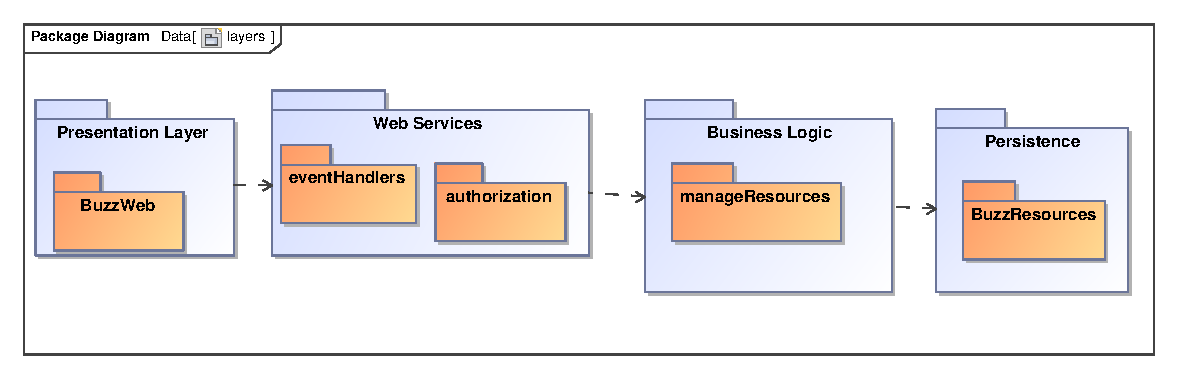
\includegraphics[width=\textwidth]{layers.eps}
\caption{Layering architecture pattern diagram \label{overflow}}
\end{figure}

%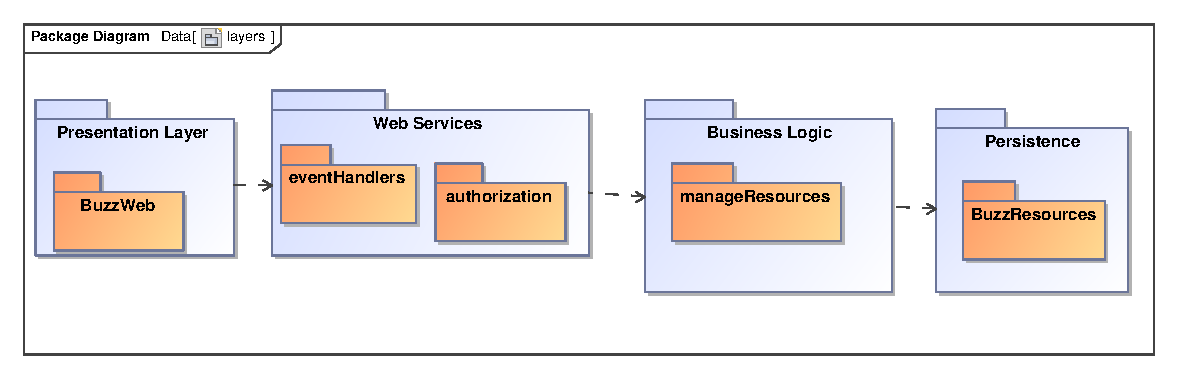
\epsfig{file=layers.eps,width=17cm}

From an MVC perspective:
%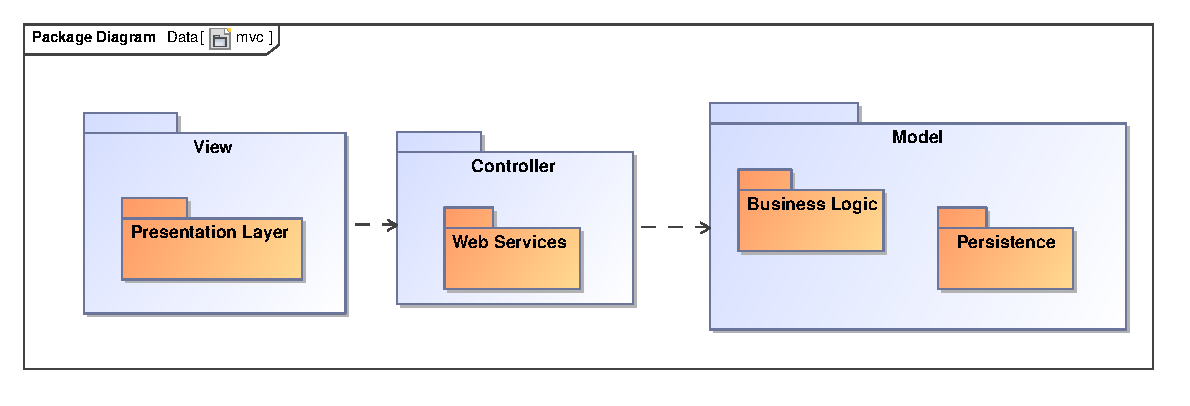
\epsfig{file=mvc.eps,width=17cm}

\begin{figure}[H]
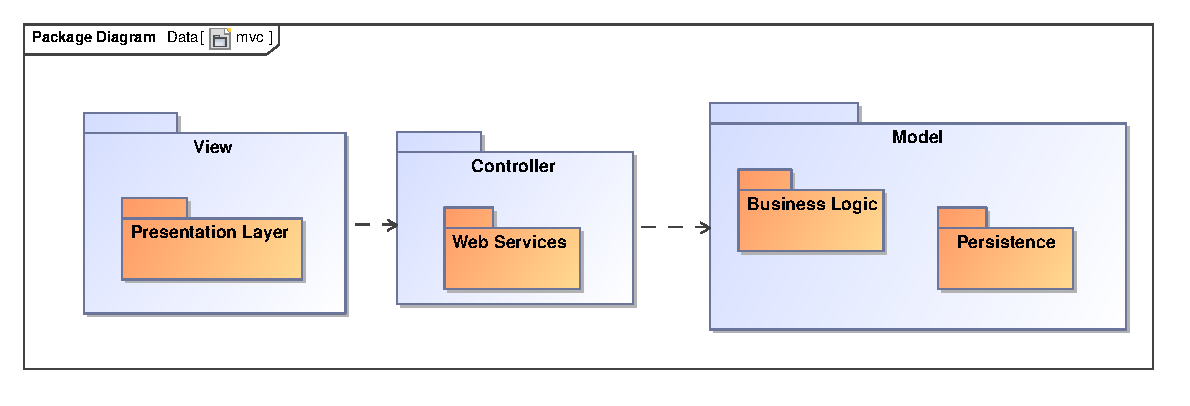
\includegraphics[width=\textwidth]{mvc.eps}
\caption{MVC architecture pattern diagram \label{overflow}}
\end{figure}


The integration between these layers will be in the form of APIs that each layer will provide to the layer directly above it.

Using the Layered pattern will improve on the following non-functional requirements:
\begin{itemize}
			\item Pluggability – different services can be tracked easily on the different layers, and can be replaced without compromising the whole system.
			\item Testability – Having different layers will make unit testing very simple since the layers are independent of each other, this implies that mock objects will be used to test each layer.
			\item Maintainability – Different teams can work on the different layers independently and maintain each layer separately.
			\item Security – Having authentication on the presentation layer and authorization in the Web services will increase security because each of these will be localized in one layer, however authentication is mostly left to LDAP.   \\[1em]
\end{itemize}


\section{Architectural Tactics or Strategies}

\section{Use of Reference Architectures and Frameworks}

\section{Access and Integration Channels}

\section{Technologies}

\section{References}

\end{document}
